\documentclass[report.tex]{subfiles}

\externaldocument{report}

\begin{document}

\section{原理・設計} \label{sec:theory}

\wfig{全体の回路図}に今回作ったAMラジオの全体図を示す。
今回作ったAMラジオは、大きく分けてラジオ回路と増幅回路からなる。
ラジオ回路は、電波から音声信号を取り出す回路である。
増幅回路は、取り出した音声信号を増幅する回路である。

\begin{figure}[H]
	\centering
	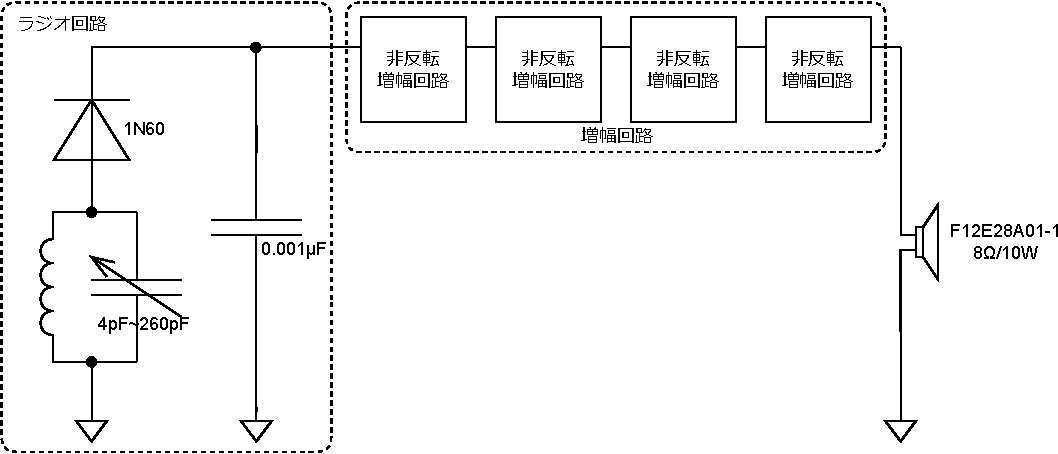
\includegraphics[width=16cm]{fig/all2.pdf}
	\caption{全体の回路図}
	\label{fig:全体の回路図}
\end{figure}

\subsection{ラジオ回路}

\wfig{radio-circuit}にラジオ回路を示す。
ラジオ回路は、電波を受信するループアンテナ、受信した電波から取り出したい周波数を選択する同調回路、受信した電波から音声周波数を取り出す検波回路からなる。

\begin{figure}[H]
	\centering
	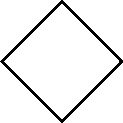
\includegraphics[width=8cm]{fig/radio.pdf}
	\caption{ラジオ回路}
	\label{fig:radio-circuit}
\end{figure}

\subsubsection{ループアンテナ}

\wfig{radio-circuit}で用いられているアンテナは、エナメル線をループ状に巻いたループアンテナである。
電波の磁界成分がループアンテナを貫くと誘導起電力(誘導電圧)を引き起こし、電流が流れる\cite{ラジオ}。
この電流を誘導電流という。
ループアンテナの誘導起電力の大きさは、\weq{induced-voltage}より求めることが出来る。
ここで、\(N[\rm{turn}]\)はループアンテナの巻数、\(\Phi[\rm{Wb}]\)は磁束、\(V[\rm{V}]\)が誘導起電力である。
\weq{induced-voltage}は、ファラデーの法則(電磁誘導の法則)に巻数\(N\)倍したものである\cite{やくにたつ}。

\begin{align}
	V = -N \frac{d\Phi}{dt} \label{eq:induced-voltage}
\end{align}

磁束\(\Phi\)は、\weq{flux}より求めることができる\cite{電磁気学}。
ここで、\(B[\rm{T}]\)は磁束密度、\(S[\rm{m^2}]\)はループアンテナの面積、\(\hat{n}\)はループアンテナの面積の法線ベクトルである。
\weq{flux}のままだと難しいため、\weq{flux2}のように単純化して考える。

\begin{align}
	\Phi = \int_S \textbf{B} \cdot \hat{\textbf{n}} dS \label{eq:flux} \\
	\Phi = B S \label{eq:flux2}
\end{align}

磁束密度\(B\)は、\weq{flux-density}より求めることができる。
ここで、\(\mu[\rm{H/m}]\)は透磁率、\(H[\rm{A/m}]\)は磁界の強さである\cite{やくにたつ}。

\begin{align}
	B = \mu H \label{eq:flux-density}
\end{align}

\weq{induced-voltage}、\weq{flux2}、\weq{flux-density}を組み合わせると、\weq{induced-voltage2}のようになる。
\weq{induced-voltage2}より、ループアンテナの誘導起電力は、磁界の強さの変化率、ループアンテナの面積、ループアンテナの巻数、透磁率に比例することがわかる。

\begin{align}
	V = -\mu N S \frac{dH}{dt} \label{eq:induced-voltage2}
\end{align}

\subsubsection{同調回路(共振回路)}

同調回路は、受信したい周波数の電波を取り出す回路である。
同調回路を用いないと、\wfig{notuse}のように、受信したい周波数の電波以外の電波も取り出してしまう。
しかし、同調回路を用いると、\wfig{use}のように、受信したい特定の周波数の電波のみを取り出すことができる。

\begin{figure}[H]
	\begin{minipage}[b]{0.5\linewidth}
		\centering
		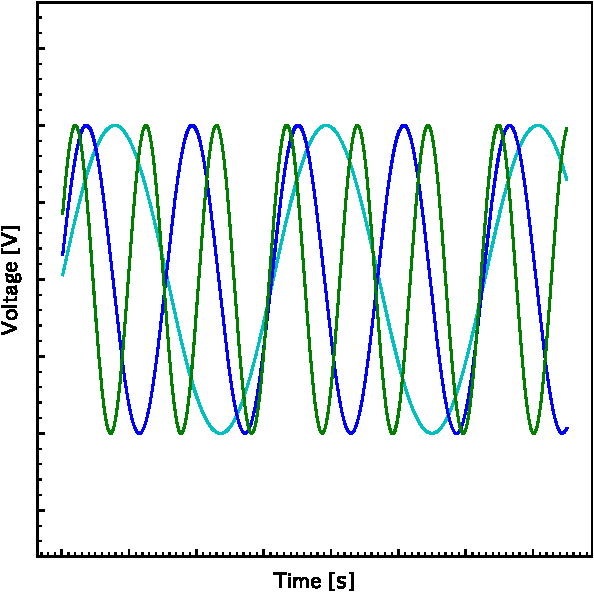
\includegraphics[width=8cm]{fig/diff.pdf}
		\caption{同調回路を用いなかった場合の受信信号}
		\label{fig:notuse}
	\end{minipage}
	\begin{minipage}[b]{0.5\linewidth}
		\centering
		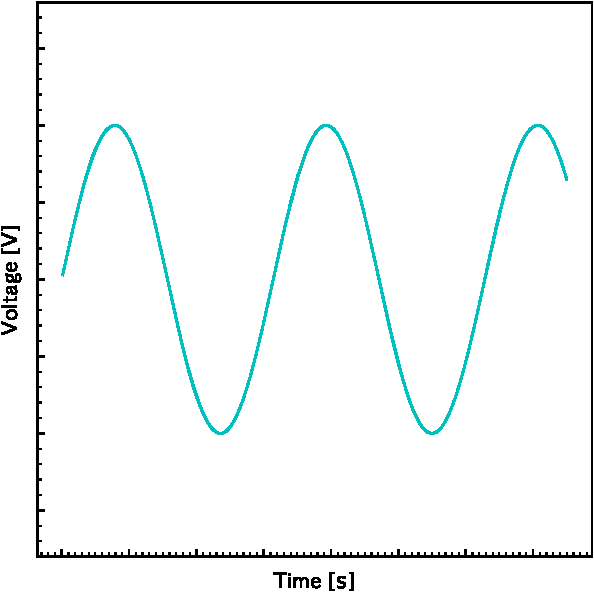
\includegraphics[width=8cm]{fig/diff2.pdf}
		\caption{同調回路を用いた場合の受信信号}
		\label{fig:use}
	\end{minipage}
\end{figure}

\subsection{同調回路の評価}

同調回路の評価として、共振周波数とQ値がある。
Q値とは、同調回路において、共振周波数以外で信号の振幅がどれほど小さいかを表す値である。
Q値が高いほど性能のよい同調回路であると言える。
Q値は\weq{Q値}で与えられる\cite{ノート}。
ここで、\(\omega_0\)は共振周波数、\(\omega_1\)と\(\omega_2\)は,振幅に共振周波数時の振幅を\(\sqrt{2}\)で割った値を取るときの周波数である(\(\omega_2 > \omega_1\))。

\begin{align}
	Q値 =\frac{\omega_0}{\omega_2 - \omega_1} \label{eq:Q値}
\end{align}

\subsubsection{理想的な同調回路}

\wfig{radio-circuit}の同調回路は、ループアンテナとバリアブルコンデンサを並列につなげている。
この同調回路の共振周波数、Q値を考えるために\wfig{kyo}のような理想的な同調回路を考える。
この並列回路のインピーダンス\(\dot{Z}\)は、\weq{impedance}のようになる。

\begin{figure}[H]
	\centering
	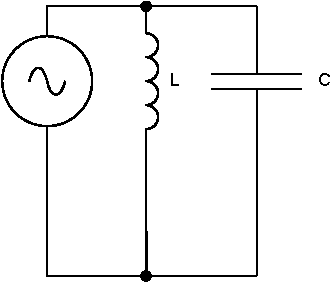
\includegraphics[width=8cm]{fig/kyo.pdf}
	\caption{理想的な同調回路}
	\label{fig:kyo}
\end{figure}

\begin{align}
	\dot{Z} & = \frac{j \omega L \times \frac{1}{j \omega C}}{j \omega L + \frac{1}{j \omega C}} = \frac{j \omega L}{1 - \omega^2 LC} \label{eq:impedance}
\end{align}

ここで、$\omega^2 LC = 1$と仮定すると、インピーダンス\(\dot{Z}\)は無限大となる。
この時の周波数(共振周波数)\(f\rm{[Hz]}\)は\weq{resonance2}\(\sim\)\weq{resonance}のようにして決定することが出来る。

\begin{align}
	\omega^2 LC & = 1                            \label{eq:resonance2} \\
	\omega      & = \frac{1}{\sqrt{LC}}                                \\
	f           & = \frac{1}{2 \pi \sqrt{LC}} \label{eq:resonance}
\end{align}

この回路のQ値は\(\infty\)である。

\subsubsection{現実的な同調回路}\label{sec:real}

また、\wfig{kyo2}のようにコイルとコンデンサの抵抗成分を考慮した現実的な同調回路を考えてみる。

\begin{figure}[H]
	\centering
	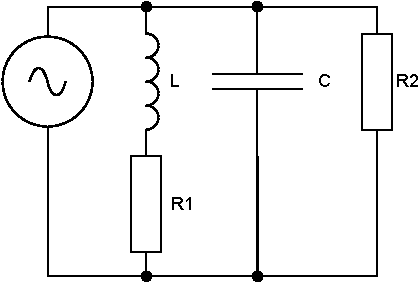
\includegraphics[width=10cm]{fig/kyo2.pdf}
	\caption{現実的な同調回路}
	\label{fig:kyo2}
\end{figure}

\wfig{kyo2}のアドミタンスは、\weq{impedance2}のようになる。

\begin{align}
	\dot{Y} & = \frac{R_1}{{R_1}^2+ {\omega L}^2} + \frac{1}{R_2} + j(\omega C - \frac{\omega L}{{R_1}^2+ {\omega L}^2})\label{eq:impedance2}
\end{align}

ここで、$\omega C - \frac{\omega L}{{R_1}^2+ {\omega L}^2} = 0$とすると、回路のアドミタンスの虚成分(サセプタンス)は0となる。
この時の周波数(共振周波数)\(f\rm{[Hz]}\)は\weq{kyousin2}\(\sim\)\weq{kyousin}のようにして決定することが出来る。

\begin{align}
	\omega C - \frac{\omega L}{{R_1}^2+ {\omega L}^2} & = 0 \label{eq:kyousin}                                                           \\
	\omega ^2                                         & = \frac{L - {CR_1}^2}{CL^2}                                                      \\
	f                                                 & = \frac{1}{2 \pi} \sqrt{\frac{1}{CL} - {\frac{{R_1}^2}{L^2}}}\label{eq:kyousin2}
\end{align}

$R_1 = 0$としたとき、\weq{kyousin}は\weq{resonance}に一致することから、正しい議論であることが分かる。
この回路のQ値は\weq{Q値2}のようになる。
\weq{Q値2}より、\(R_2\)が高い、\(R_1\)が低いほどQ値が高くなることが分かる。

\begin{align}
	Q = \frac{\omega_0 L R_2}{R_2R_1 + (\omega_0 L)^2} = \frac{\omega_0 L}{R1 + \frac{(\omega_0 L)^2}{R_2}} \label{eq:Q値2}
\end{align}

\wfig{全体の回路図}では、ループアンテナのインダクタンス\(L\)を変更することができない。
そのため、バリアブルコンデンサのキャパシタンス\(C\)を変更することで、受信したい周波数を選択する。

\subsubsection{混信率}

\weq{混信率2}\weq{混信率}に、Aラジオ局がBラジオ局にどのぐらい混信してしまうのかを示す。
混信率が高いと、Aラジオ局とBラジオ局の両方を受信してしまい、複数の音声が聞こえてしまう。
ここで、\(f_A\)と\(f_B\)はAラジオ局、Bラジオ局の周波数を示す\cite{ノート}。

\begin{align}
	k   & = \frac{\omega_A}{\omega_B} = \frac{f_A}{f_B} \label{eq:混信率2}                                                                                         \\
	混信率 & = \frac{1}{\sqrt{1 + \left(k + \frac{1}{k}\right)^2 Q^2}} = \frac{1}{\sqrt{1 + \left(\frac{f_A}{f_B} + \frac{f_B}{f_A}\right)^2 Q^2}}  \label{eq:混信率}
\end{align}

\subsubsection{選択する周波数} \label{sec:select}

\wfig{map}にAMラジオの送信所を地図にそれぞれ示したものを示す。
\wtab{zyushin}にAMラジオの送信所の一覧とその周波数、送信出力、学校までの距離、地図上の色(数字)を示す。
ここで、\wfig{map}の黒と桃色で作られた四角形は、受信場所である学校の大まかな場所を示している。
(受信をテストした教室を基準に考えると)黒は壁でかこまれ、桃色は窓である。
\wfig{map}でピンが刺さっている場所は、AMラジオの送信所でそれぞれ\wtab{zyushin}に対応している。

\begin{figure}[H]
	\centering
	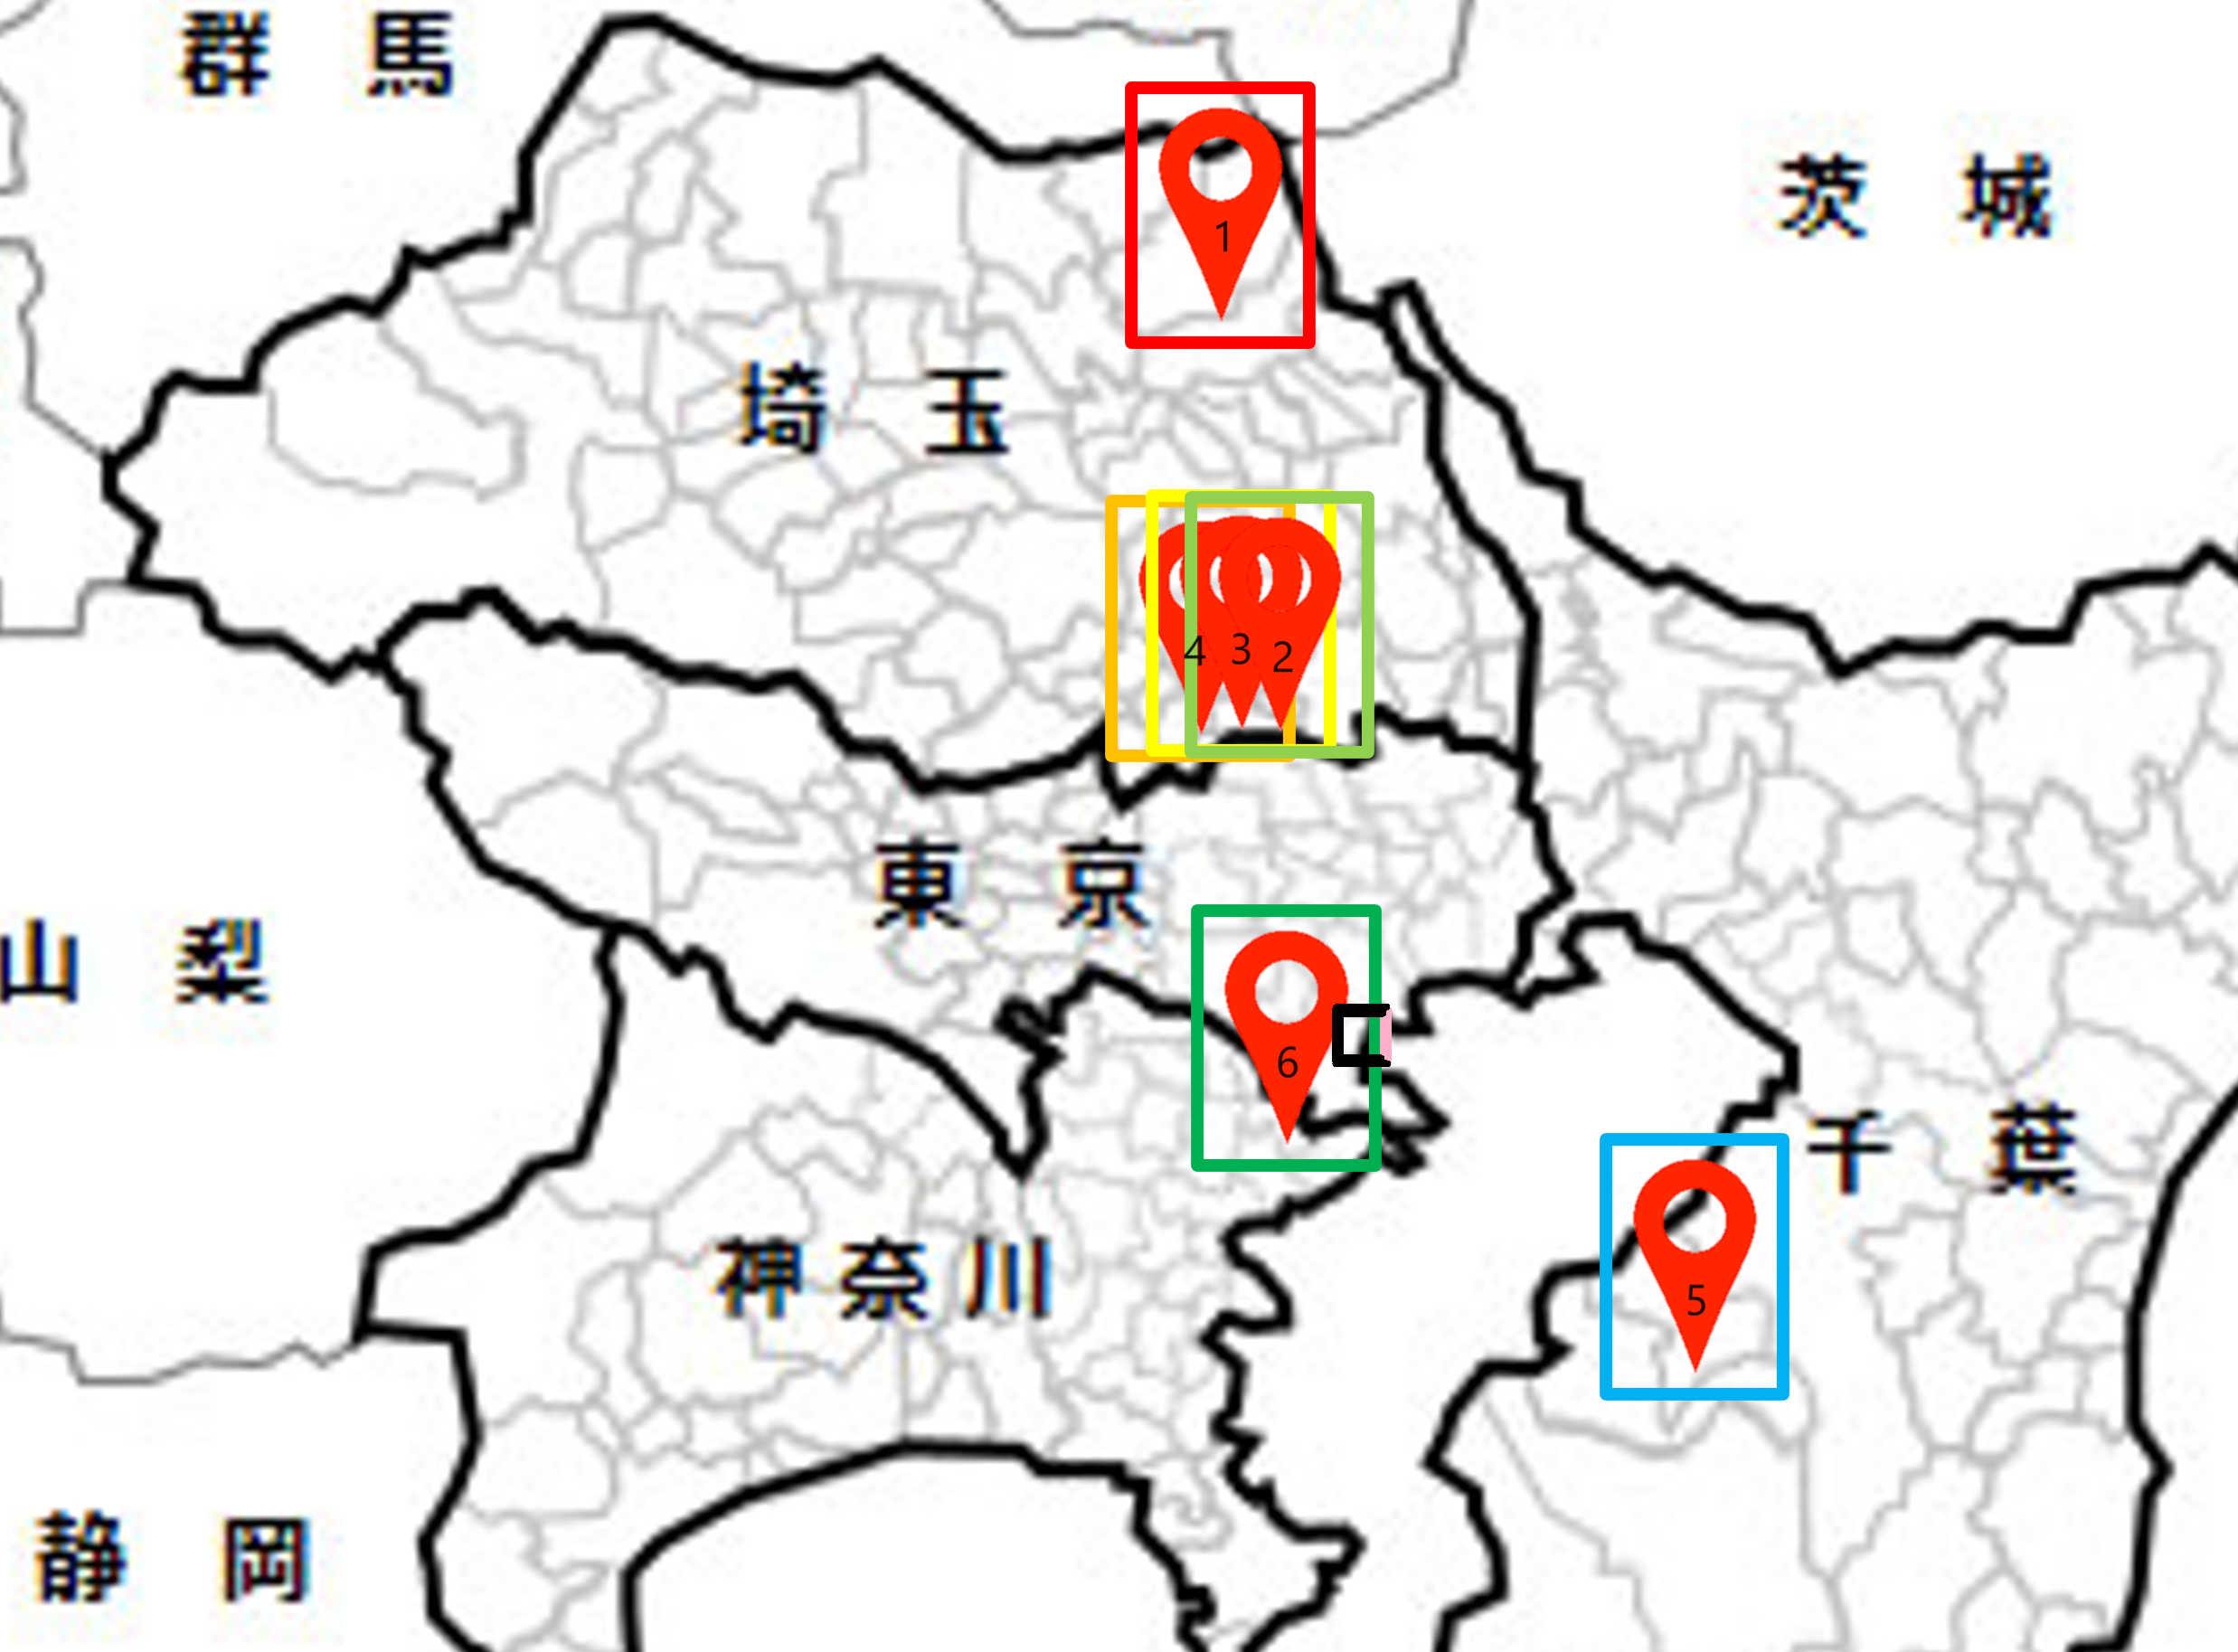
\includegraphics[width=15cm]{use/map.png}
	\caption{AMラジオの送信所の地図}
	\label{fig:map}
\end{figure}

\begin{table}[H]
	\centering
	\caption{AMラジオの送信所(東京で受信できると考えられる局)}
	\label{tab:zyushin}
	\begin{tabular}{ccccc} \hline
		放送局    & 周波数[kHz] & 送信出力[kW] & 学校までの距離[km] & 地図上の色(数字) \\ \hline
		NHK第1  & 594      & 300      & 約52.6       & 赤(1)      \\
		NHK第2  & 693      & 500      & 約52.6       & 赤(1)      \\
		AFN    & 810      & 50       & 約22.4       & 黄緑色(2)    \\
		TBSラジオ & 954      & 100      & 約23.6       & 黄色(3)     \\
		文化放送   & 1134     & 100      & 約24.3       & 橙色(4)     \\
		ニッポン放送 & 1242     & 100      & 約31.8       & 水色(5)     \\
		ラジオ日本  & 1422     & 50       & 約7.8        & 緑色(6)     \\ \hline
	\end{tabular}
\end{table}

\subsubsection{レーダー方程式}

レーダー方程式を\weq{radar}に示す。なおこれは,反射やアンテナゲインを考慮していない簡易的なものである。
\weq{radar}を用いると電力密度を計算することができる。
ここで、\(R\)は送信場所から受信場所までの距離、\(P_t\)は送信電力である。

\begin{align}
	電力密度 = \frac{P_t}{4 \pi R^2} \label{eq:radar}
\end{align}

\subsubsection{検波回路}

検波回路は、電波から受け取った信号から音声信号を取り出す回路である。
今回作ったAMラジオが受信するのは、振幅変調波(AM波)である。
振幅変調波は、\wfig{5V}のような搬送波と、\wfig{3V}のような信号波を用いて、\wfig{wave}のような波を電波として送信される。
仮に、搬送波\(v_c\)の振幅を\(V_{cm}\)、周波数を\(f_c\)、信号波\(v_s\)の振幅を\(V_{sm}\)、周波数を\(f_s\)とすると、それぞれ\weq{v_c}\weq{v_s}のように表すことができる\cite{電子回路}。

\begin{align}
	v_c = V_{cm} \sin(2 \pi f_c t) \label{eq:v_c} \\
	v_s = V_{sm} \sin(2 \pi f_s t) \label{eq:v_s}
\end{align}

\begin{figure}[H]
	\begin{minipage}[b]{0.5\columnwidth}
		\centering
		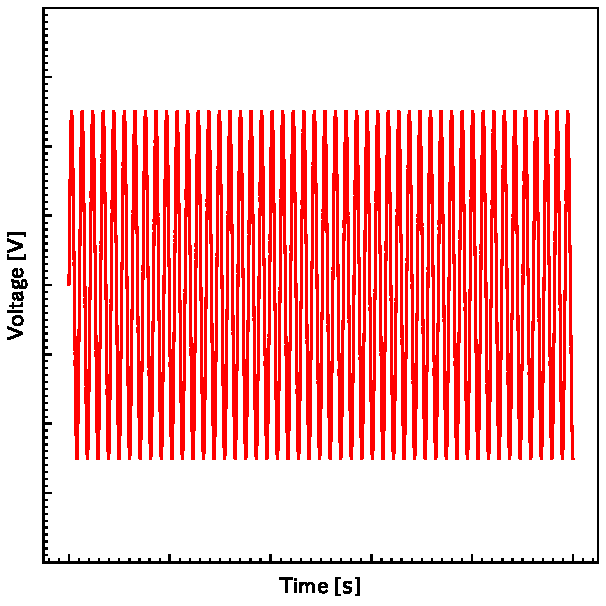
\includegraphics[width=7cm]{fig/5V.pdf}
		\caption{搬送波}
		\label{fig:5V}
	\end{minipage}
	\begin{minipage}[b]{0.5\columnwidth}
		\centering
		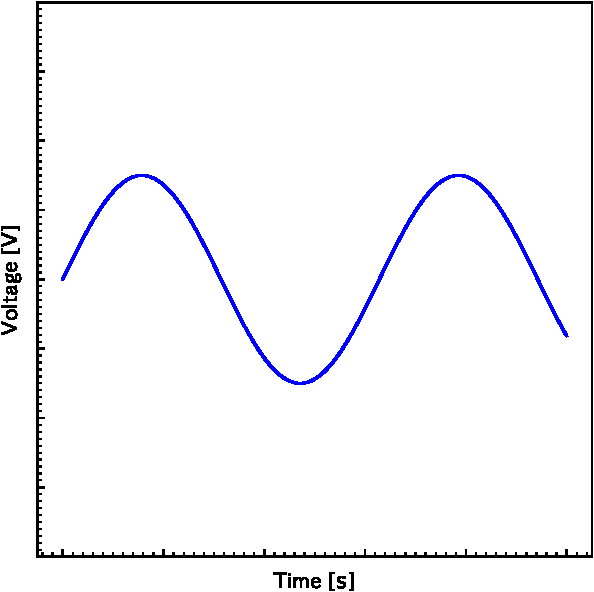
\includegraphics[width=7cm]{fig/3V.pdf}
		\caption{信号波}
		\label{fig:3V}
	\end{minipage}
\end{figure}

振幅変調波\(v_o\)は、\weq{v_o}で表すことができ、\wfig{wave}のような波形になる。

\begin{align}
	v_o = (V_{cm} + V_{sm} \sin(2 \pi f_s t)) \sin(2 \pi f_c t) \label{eq:v_o}
\end{align}

\begin{figure}[H]
	\centering
	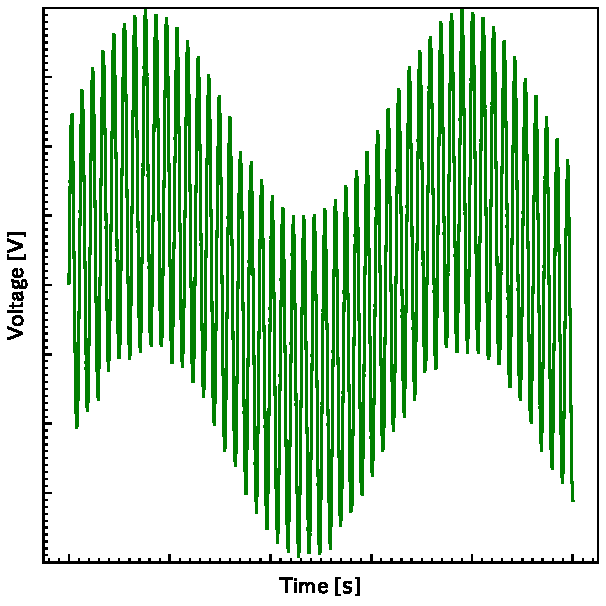
\includegraphics[width=7cm]{fig/Wave.pdf}
	\caption{電波から受信された信号(振幅変調波)}
	\label{fig:wave}
\end{figure}

\wfig{radio-circuit}の検波回路ではまず、ゲルマニウムダイオードを用いて、\wfig{wave}から\wfig{diode}のような波形にする。
ダイオードには、順方向特性(逆方向に電圧がかからない)があるため、電圧がマイナスになっている部分はカットされる\cite{電子回路}。

\begin{figure}[H]
	\centering
	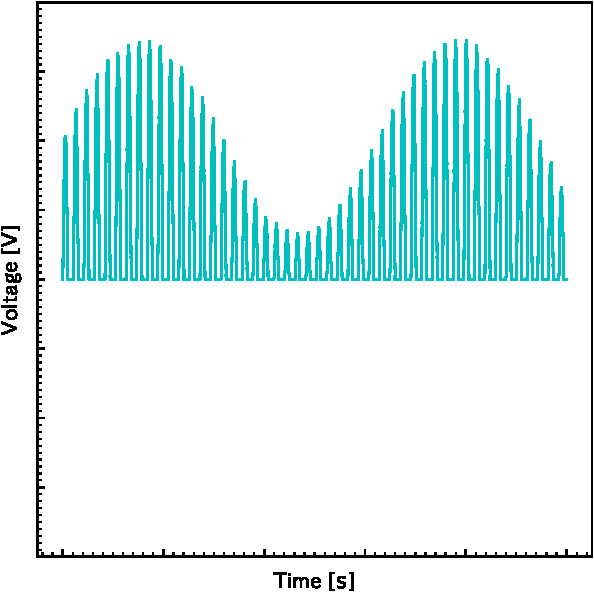
\includegraphics[width=7cm]{fig/diode.pdf}
	\caption{ダイオードで逆方向電圧を取り除いた信号}
	\label{fig:diode}
\end{figure}

また、0.001\(\upmu\)Fのコンデンサを用いて、搬送波部分を取り除く。
キャパシタンスは、搬送波のような高い周波数に対しては、インピーダンスが小さくなる。
逆に、信号波のような低い周波数に対しては、インピーダンスが大きくなる。
そのため、\wfig{diode}から\wfig{capa}のように搬送波が取り除かれて、信号波のみが残る。
この時、多少バイアス電圧がかかっている。

\begin{figure}[H]
	\centering
	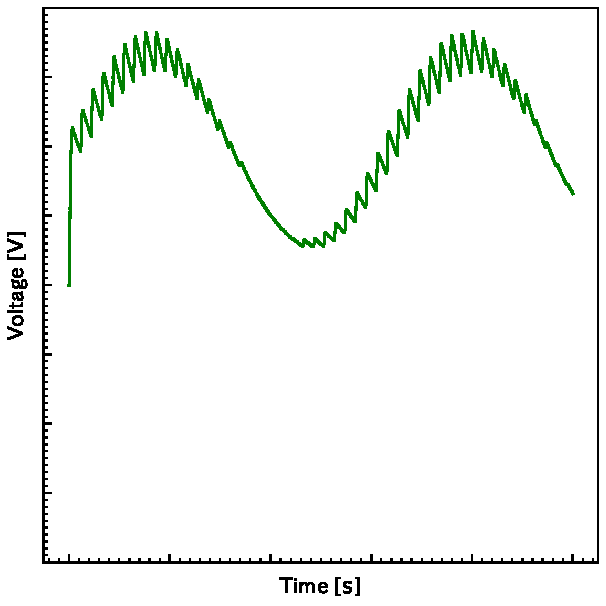
\includegraphics[width=7cm]{fig/capa.pdf}
	\caption{キャパシタンスで搬送波部分を取り除いた信号}
	\label{fig:capa}
\end{figure}

\subsection{増幅回路}

\wfig{amplifier-circuit}に実際に作成した増幅回路を示す。
\wfig{amplifier-circuit}は、\wfig{amplifier-circuit2}のような非反転増幅回路をベースにして設計されている。

\begin{figure}[H]
	\centering
	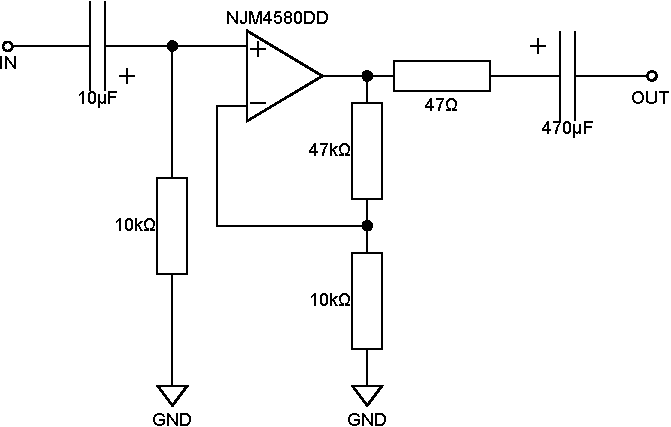
\includegraphics[width=15cm]{fig/amp.pdf}
	\caption{実際に作成した増幅回路}
	\label{fig:amplifier-circuit}
\end{figure}

\begin{figure}[H]
	\centering
	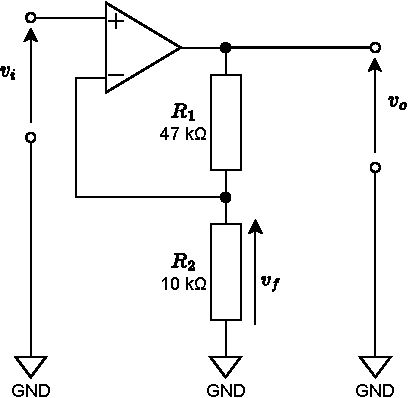
\includegraphics[width=8cm]{fig/amp2.pdf}
	\caption{非反転増幅回路}
	\label{fig:amplifier-circuit2}
\end{figure}

\subsubsection{非反転増幅回路}

\wfig{amplifier-circuit2}を用いて増幅度を考える。
まず、オペアンプ(演算増幅器)の入力インピーダンスは、無限大であると仮定する(つまり理想的なオペアンプ)。
差動入力電圧は、(\(v_i - v_f\))である。
そのため、出力電圧\(v_o\)は\weq{amp}のようになる。
この時、\(A_v\)はオペアンプの増幅度を示す。

\begin{align}
	v_o = A_{v} (v_i - v_f) \label{eq:amp}
\end{align}

帰還電圧\(v_f\)は、\(R_1\)と\(R_2\)の分圧により\weq{amp2}のようになる。

\begin{align}
	v_f = \frac{R_2}{R_1 + R_2} v_o \label{eq:amp2}
\end{align}

\weq{amp}に\weq{amp2}を代入すると、\weq{amp3}\(\sim\)\weq{amp4}のようになる。

\begin{align}
	v_o & = A_v \left( v_i - \frac{R_2}{R_1 + R_2} v_o \right) \label{eq:amp3}               \\
	v_o & = \frac{A_v}{\frac{A_v R_1}{R_1 + R_2}} v_i                                        \\
	v_o & = \frac{1}{\frac{1}{A_v} + \frac{R_1}{R_1 + R_2}} v_i              \label{eq:amp4}
\end{align}

ここで、\(A_v = \infty\)であると仮定すると、\weq{amp5}のようになる。

\begin{align}
	v_o = \frac{R_1 + R_2}{R_1} v_i \label{eq:amp5}
\end{align}

\weq{amp5}から、電圧増幅度\(A_{vf}\)を求めると\weq{amp6}のようになる。

\begin{align}
	A_{vf} = \frac{v_o}{v_i} = \frac{R_1 + R_2}{R_1} = 1 + \frac{R_2}{R_1} \label{eq:amp6}
\end{align}

よって、\wfig{amplifier-circuit2}の電圧増幅度は、\weq{amp7}のようになる\cite{電子回路}。

\begin{align}
	A_{vf} = 1 + \frac{47\rm{k}}{10\rm{k}} = 5.7倍 \label{eq:amp7}
\end{align}

\subsubsection{実際に作成した増幅回路}

\wfig{amplifier-circuit}は、\wfig{amplifier-circuit2}にいくつか素子を加えている。
まず、\wfig{amplifier-circuit}の\(C_1\)と\(C_2\)は、直流電圧をカットするためのカップリングコンデンサである。
コンデンサは、高周波数に対してはインピーダンスが小さくなるため、直流は通さない。
カップリングコンデンサをつける理由として、交流成分に直流成分が含まれてしまうと、オペアンプの電源として用いてる9Vよりも最大電圧が高い電圧(-9Vよりも最低電圧が低い電圧)を出力しようとしてしまうことがよくある(直流がない場合でもあるが可能性的に直流がある場合と比較して低い)。
正弦波を入力していたと仮定すると、上半分(もしくは下半分)だけが方形波のようになってしまい、波形が歪んでしまう。
また、スピーカーに直流成分をかけてしまうと、スピーカーが壊れてしまうことがある。
\(C_3\)と\(C_4\)は、オペアンプの電源として用いている電池から発生するノイズをカットするためのバイパスコンデンサである。
\(R_3\)の抵抗は、短絡してはいけない部分(電源やグラウンドなど)が短絡して過電流が流れないようにするための保護抵抗である。
\(R_4\)の抵抗は、オペアンプを正常に動作させるためのバイアス抵抗である。
\(R_4\)の抵抗を挿入することによって、無信号時に入力をGNDに固定することができる。
また、\(R_4\)の抵抗がオペアンプの入力インピーダンスの代わりになってくれるためバイアス電流が流れやすくなる。

\subsection{可変抵抗(ボリューム)}

可変抵抗には、主にAカーブとBカーブとCカーブなどの種類がある。
\wfig{cabe}にそれぞれのカーブの特性を示す。
Aカーブは、回転角度に対して、抵抗値が指数関数的に上昇する。
Bカーブは、回転角度に対して、抵抗値が比例的に上昇する。
Cカーブは、回転角度に対して、抵抗値が対数関数的に上昇する。
人間の耳は、オーディオの出力信号に対して比例的に感じることはなく、その対数に比例して感じる(小さい音に敏感に反応する)。
そのため、オーディオの音量調節には、Aカーブの可変抵抗を用いるのが良い。

\begin{figure}[H]
	\centering
	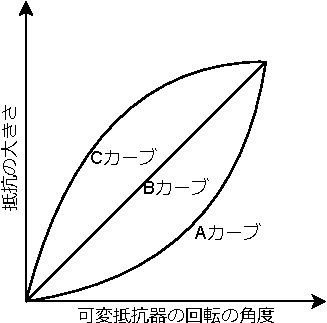
\includegraphics[width=7cm]{fig/cabe.pdf}
	\caption{可変抵抗のカーブ}
	\label{fig:cabe}
\end{figure}

\end{document}
